% CHAPTER 1 LESSON 3
\clearpage
\section{Source Filter Model}
\label{Source Filter Model}

The previous lesson introduced the method by which we produce speech. The lungs produce energy, in the form of airflow, that passes through the larynx where either oscillating vocal chords produce voiced speech or the airflow simply passes through to produce unvoiced speech.  This energy then passes through vocal tract, where the current positioning of the jaw, lips, tongue, etc. affect the shape and therefore the speech sound that is uttered.  This process can be modeled by a source filter model.  This assumes that we have a source, the airflow after it passes through the larynx, and then a filter which is defined by the resonance frequencies of the vocal tract. In this model, we assume that these two are independent. This is a very critical assumption and important to understand and would require, for example, that the resonances of the vocal tract are independent of the fundamental frequency of the excitation. The ultimate goal is to model this process mathematically and for this we have to understand what is really going on in the process. \\

\begin{wrapfigure}{l}{0pt}
    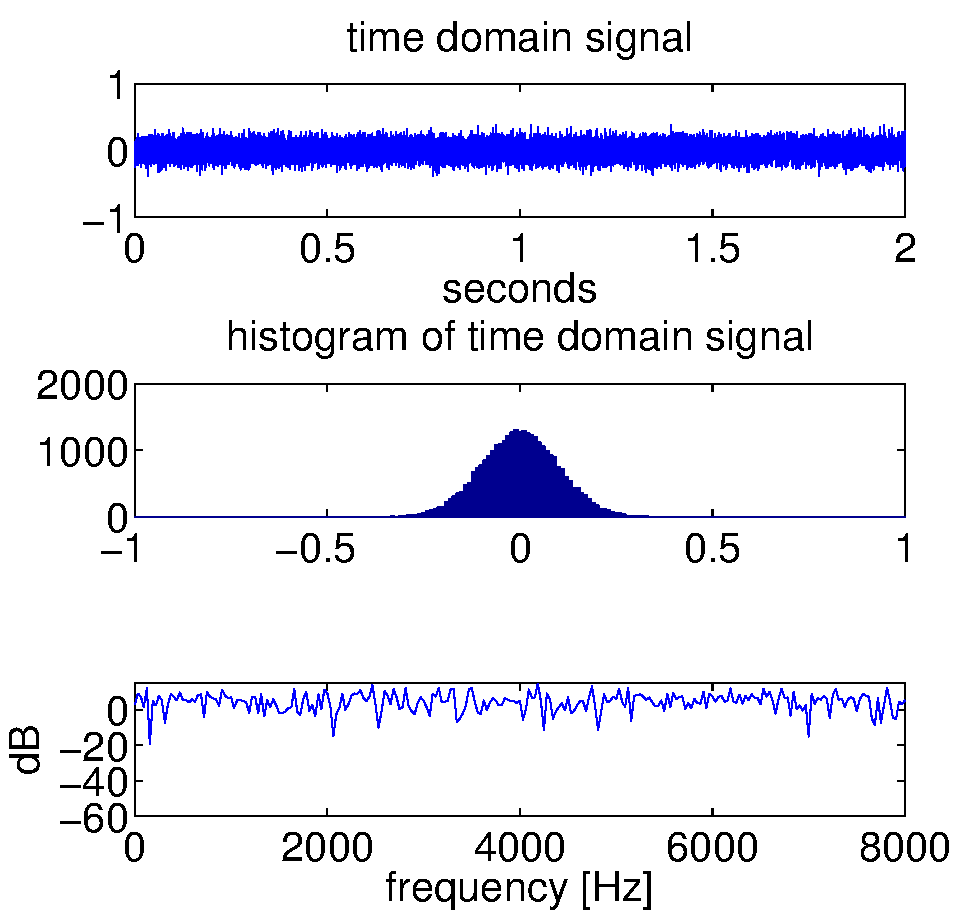
\includegraphics[width=0.5\textwidth]{Pictures/Chapter1_Lesson3/gaussianNoise-eps-converted-to.pdf}
    \caption{Statistics of white Gaussian noise.}
    \label{gaussNoise}
\end{wrapfigure}

The excitation signal for a unvoiced sounds is described  by turbulent airflow passing through the glottis. This can be modeled by using white Gaussian noise. The top of fig \ref{gaussNoise} depicts the time domain signal of white Gaussian noise. It is Gaussian noise, because a histogram of the samples in the signal will produce a Gaussian distribution. As can be seen in the histogram, there are more values close to zero than there are towards the edges. It is white noise, because a Fourier transform of the signal produces a flat spectrum.  The term ''white'' refers to a flat spectrum because in optics, white light as composed of an equal amount of energies of all frequencies, whereas light that has more energy in lower frequencies would be red.\\



For a voiced excitation, the vocal chords open and close periodically. If we look at the glottal flow behind the larynx, what is observed is a periodic form. First, we start with closed vocal chords, a closed glottis. Next, as we produce energy with our lungs, we push air and the glottis opens because there is an increased pressure that builds up at the base. As the glottis opens, the pressurized air can now escape and the thus, the airflow increases and by Bernoulli's principle, the pressure decreases. Because the vocal chords are under tension, this decrease in pressure allows them to snap shut to begin the process again. This is the mechanism behind voiced excitation. \\

\begin{wrapfigure}{l}{0pt}
    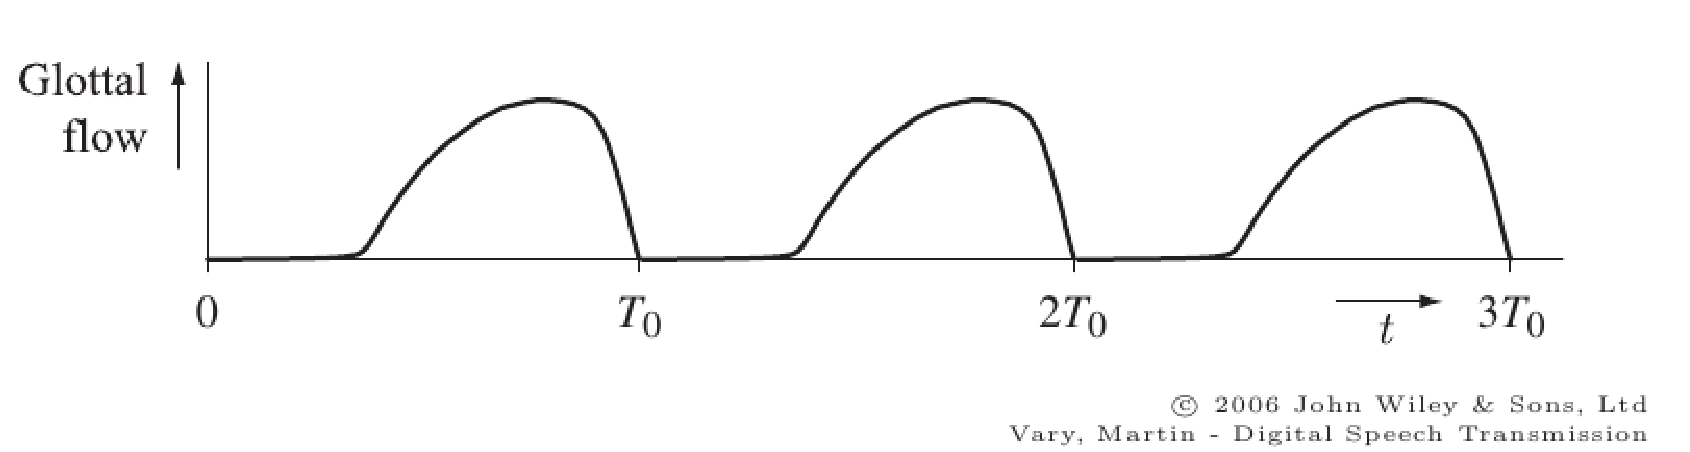
\includegraphics[width=0.5\textwidth]{Pictures/Chapter1_Lesson3/glottalFlow-eps-converted-to.pdf}
    \caption{Glottal flow over time}
    \label{glotFlow}
\end{wrapfigure}

 The two forms of excitation can now be described in a simple model. In the unvoiced case,  a noise generator can be used to produce the excitation energy.  For voiced speech, a pulse train in the time domain can be used with a peak to peak distance of the fundamental period, \begin{math}T_0\end{math} This will model the opening and closing of the glottis.  It is then necessary to have a switch that chooses between the two forms of excitation and some form of detector that can determine which excitation is present in the current speech signal.  There are also mixed excitation sounds, so one could also imagine there being a weighted summation of the two excitation signals, so we could have something that's a little more complicated like a weited summation to produce mixed excitation signals. \\

The next step is to model the vocal tract as a filter through which the excitation signal passes. The vocal tract can be thought of as a filter because it will have certain resonance frequencies similar to the resonances of a tube. In fact, the vocal tract can be simplified by using a tube model in which there is one input and two outputs, the lips and the nose. This can be seen in fig \ref{tubeModel}, where the tube on the bottom represents the oral cavity with another tube on top representing the nasal cavity.  The tubes will be separated by a switch that models the vallum.  Each tube will have its own resonance.  By modifying the shape of the tube, different resonances would be produced thus producing different speech sounds .\\

\begin{wrapfigure}{l}{0pt}
    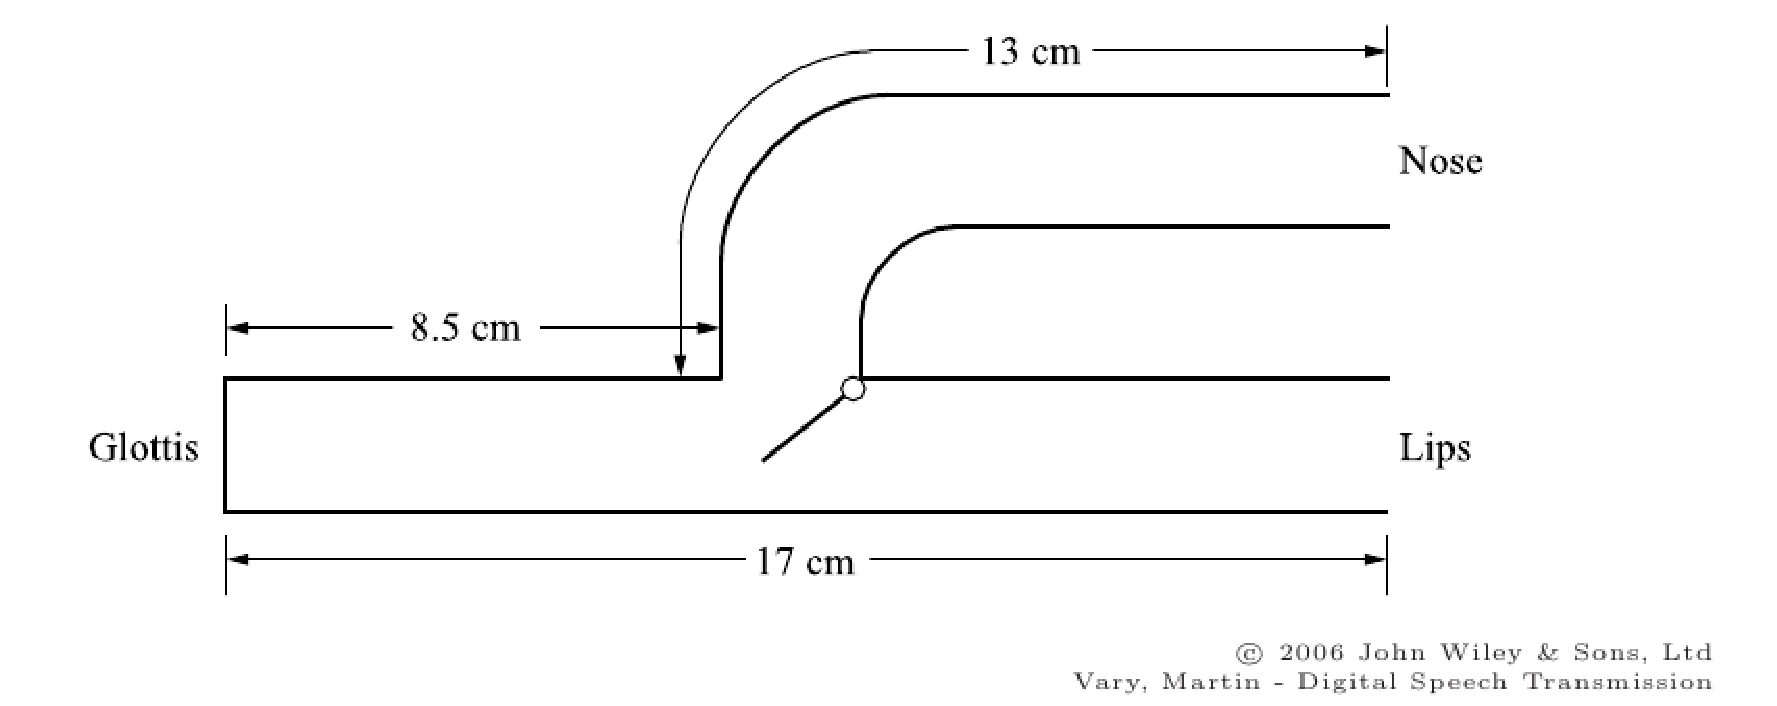
\includegraphics[width=0.7\textwidth]{Pictures/Chapter1_Lesson3/vocalTractSimple1-eps-converted-to.pdf}
    \caption{Simplified model of the vocal tract.}
    \label{tubeModel}
\end{wrapfigure}

From a signal processing view, the vocal tract filters the excitation signal to produce a speech sound. Mathematically speaking, this is represented by a convolution in the time domain and a multiplication in the frequency domain. The vocal tract can therefore be thought of as a transfer function. The spectrum of this transfer function would contain certain resonances. This can be seen in fig \ref{transFunc}. In signal processing, these are called formants, the resonances of the vocal tract. Formants contain important information because they decide what speech sound is being produced.  When the spectra of the excitation signal and the vocal tract transfer function are multiplied, what is seen is the result of what would happen if we did a frequency analysis of a recorded speech sound. The influence of the excitation signal and the vocal tract can both be seen in the final signal. It is very important to understand that these are two independent signals in our model. Notice that at the bottom of fig \ref{transFunc}, the formant peak is not seen. It lies between the two peaks of the harmonics because the final signal is an almost sampled version of the vocal tract function. Babies are very skilled at aligning the fundamental frequency with the formant, because this is when they scream the loudest! If the harmonics are between the peak of the formants, the energy in the final signal would be lower as opposed to the harmonic being aligned with the formant.  The peaks of the formants are given by the multiple peaks seen  in the transfer function, whereas the fundamental frequency is given by the first peak of the fine structure or the distance between two neighboring peaks.\\

\begin{wrapfigure}{l}{0pt}
    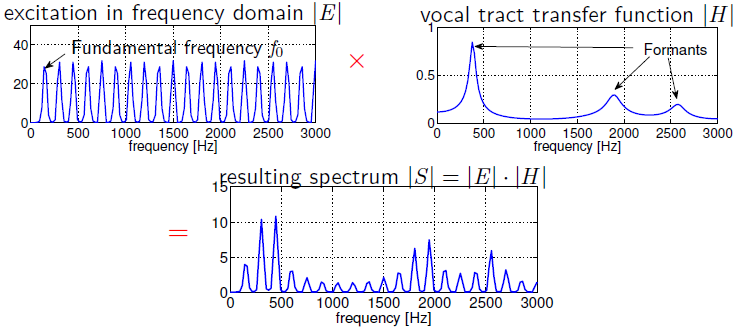
\includegraphics[width=0.7\textwidth]{Pictures/Chapter1_Lesson3/Transferfunc.png}
    \caption{Transfer function of the vocal tract.}
     \label{transFunc}
\end{wrapfigure}

Formant freq vs fundamental freq.  
Formants are imporatnt becasue they define the meaning of a speech sound.

We can then draw a formatn map with this information.  If we look at the map, we can see a caertain area  where phonemens have their formants. How lare the area is depends on the database used to create it .

It is imporant to understand the difference between fundamental frequecny and formants.  The formants carry the meaning where as the fundamental frequency refers to the excitiation signal and carries no real meaning (only with respect to tintonation prosody)

So for simple model of speech production there are certain parameters taht we need to know.  We would need to know: voiced/unvoiced speech signal to switch our excitiation and for this one, we would need to know our fundamental period, and our voacl tract transfer function.

